\section{Linear Regression}

Linear Regression is a common technique in the world of predictive analytics. One common example of linear regression is the fitting of straight lines to a graph. 

[INSERT IMAGE]

Is a supervised machine learning technique [EXPAND]

The data is usually not perfect, there is often a source of noise, this could be network latency

\begin{equation}
    f(x) = mx+c
\end{equation}

This describes a straight line relationship, where y is the y axis variable and x is the x axis variable, the relationship between them is defined as m where m is the slope of the line. c is a constant or intercept where the line meets the y axis

The above image is an example of building a model with one variable, which predicts y based on the values of x using an intercept and slope values. More generally we will be fitting muliple co-efficients. Co-efficients means lots of different features. For example if we want to predict weather, then to make an accurate model we would probably need multiple features such as wind speed and atmospheric pressure.

\begin{equation}
\hat{y} = \frac{1}{n}\sum_{i=1}^n y_i
\end{equation}

Y hat is the predicted value of y. Beta 0 corresponds to to the intercept value. Sum of, is iterating over the features denoted by k. k can be described as the k co-efficient values for a feature.[EXPAND]

\subsection*{Linear Regression Features}

Linear regression works by finding a straight line relationship between a set of features (coefficients). Features could be anything from miles per gallon of a new car to the frequency of a cpu. One caveat with these features is that in linear regression they must be expressed numerically. For example if we have a feature x which denotes the gender of a human as either 'M', 'F'. We could can not input these values into our regression as they are not numeric. These values could not be used in our regression without being transformed. One of the methods of data transformation is called one hot encoding. 

\subsection*{Feature Transformations}

There are certain cases where a feature transformation is required. As mentioned earlier we would need one hot encoding to make sure our data is numeric. Using our example of a gender feature above, one hot encoding will take the string values 'M' and 'F' and convert them to numbers. Interestingly it will not replace our gender column, instead it will create 2 more features. We will end up with a new male and female feature encoded with a 1 for a true value and a 0 for a false value.

[NEEDS IMAGE OF ONE HOT ENCODING]

Transformations can be used to account for a non-linear relationship between our features and the predictor. Non linear relationships can be difficult to find, and usually relies on a deep understanding of the the data. Once we have this understanding we can start to ask questions such as, can the slope of
the relationship between Xi and E(Y) be expected to have the same sign for all values of Xi. Should we expect the magnitude of the slope to increase as Xi increases, or should we expect
the magnitude of the slope to decrease as Xi increases?\cite{nonlinearRelationships}

\subsection*{Residuals vs fits plot}

One way to detect non linearity in a dataset is to use a residuals vs fits plot. It is a scatter plot of residuals on the y axis and fitted values (estimated responses) on the x axis. The plot is used to detect non-linearity, unequal error variances, and outliers \cite{residualsVsFitsPlot}. this residual plot may be used to check for violations in model assumptions particularly related to incorrect specification or presence of heteroscedasticity\cite{doi:10.1002/9781118625590.ch2}. Lets look at a simple linear regression model

\[ Y = \beta_0 + \beta_1X + \epsilon \]

The error terms are assumed to be normally distributed, homoscedastic(every value has the same variance) and are  independant of one another. If these assumtptions are correct than the observered residuals should be aproxamatly normally distributed with constant variants for all the X values.

\begin{figure}[H]
  \centering
  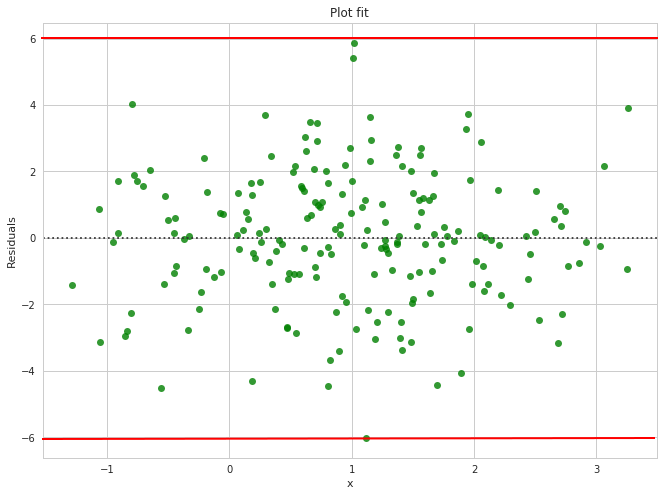
\includegraphics[scale=0.5,width=100mm]{./images/plotfit-good.png}
  \caption{Fit plot showing a good indication that the assumptions of our model are correct}
  \label{fig:fitsplotgood}
\end{figure}

In figure \ref{fig:fitsplotgood} we can see that variablity is roughly the same for all the different values of X between the 2 red lines. There also does not appear to be much curvature or any other indications that there is a problem with our model. figure \ref{fig:fitsplotgood} gives us no indication that the assumptions of our model are false


\begin{figure}[H]
  \centering
  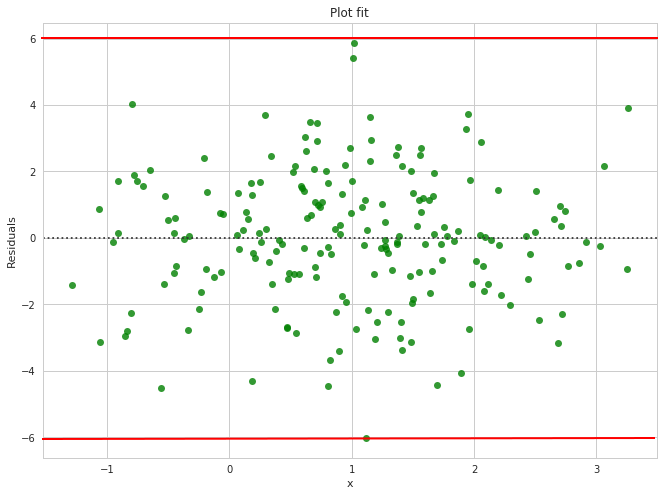
\includegraphics[scale=0.5,width=100mm]{./images/plotfit-good.png}
  \caption{Fit plot showing a good indication that the assumptions of our model are correct}
  \label{fig:fitsplotbad}
\end{figure}

[FIND A REAL IMAGE REFERENCE - https://www.youtube.com/watch?v=iMdtTCX2Q70]

In figure \ref{fig:fitsplotbad} there are more odvious problems. The variants of the residuals increases with the x axis. This would be considered a violation of our constant variable assumption. One option to deal with this situation is to use a technique called weighted regression. However overall our model assumptions are incorrect for this model.

\subsection*{Measuring Model Errors}

If we are using linear regression to predict values, then we will need to measure the errors to prevent overfitting or underfitting.
\begin{figure}[H]
  \centering
  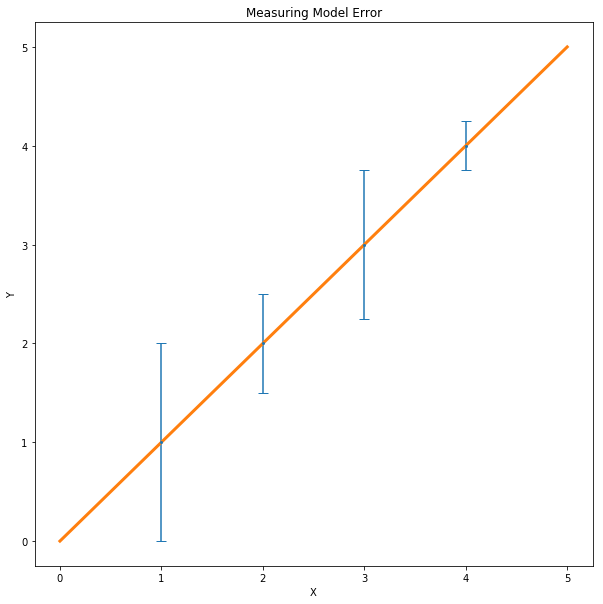
\includegraphics[scale=0.5,width=100mm]{./images/graph-error-bars.png}
  \caption{Fit plot showing a good indication that the assumptions of our model are correct}
  \label{fig:graph-error-bars}
\end{figure}
In figure \ref{fig:graph-error-bars} we can see a linear model graph showing error levels. Each vertical bar represents some degree of an error. The further away from the straight orange line the greater the error. We can use the formula below to determine the error for each bar.
\begin{equation}
    \epsilon_i = y_i - \hat y_i
\end{equation}
Generally speaking if the error is less than zero this means that we have overestimated the values. If the error is greater than zero than the prediction is less than the true value. If our error is zero than it can be considered accurate.

The equation mentioned above is good when dealing with single values. However if we have a dataset with many features it may be more usefull to measure the errors with a historgram.

\begin{figure}[H]
  \centering
  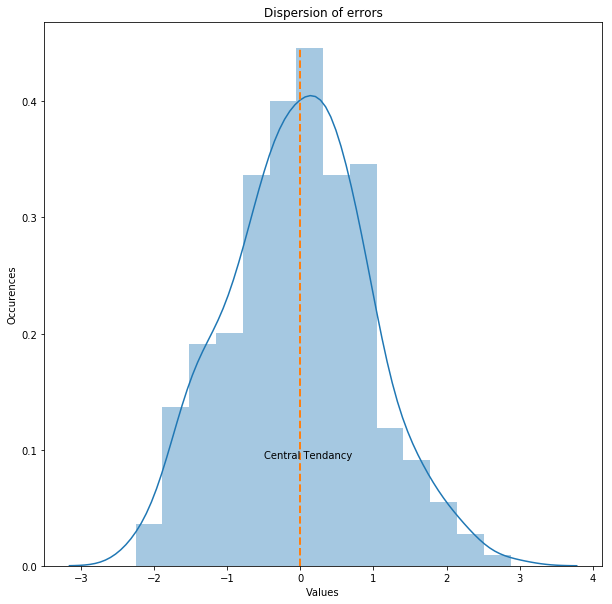
\includegraphics[scale=0.5,width=100mm]{./images/graph-histogram.png}
  \caption{Fit plot showing a good indication that the assumptions of our model are correct}
  \label{fig:graph-histogram}
\end{figure}
Figure \ref{fig:graph-histogram} shows a histogram which could be used for multiple features. The dashed orange line is called the central tendancy. We can see that this particular graph is showing that errors will occur between -2.2 and +2.9, this is known as the dispersion of errors.

\subsection*{Advantages of linear regression}

Linear regression is a relatively simple to understand when compared to other prediction techniques such as deep neural networks.

Predictor importance can be measured by its coefficients. For example if we have 10 coefficients it is possible to measure the importance of each feature towards to the final prediction. To measure this we can look at how large the coefficient is compared to the target variable.

We can apply certain transformations on our data to come up with 


\subsection*{Least Squares}
\subsection*{K Nearest Neighbours}
\subsection*{Ridge Regression}
\subsection*{Lasso Technique}

\subsection*{Shrinkage Methods}